%%%%%%%%%%%%%%%%%%%%%%%%%%%%%%%%%%%%%%%%%%%%%%%%%%%%%%%%%%%%%%%%%%%%%%%%%
%%%%%%%%%%%%%%%%%%%%%%%%%%%%%%%%%%%%%%%%%%%%%%%%%%%%%%%%%%%%%%%%%%%%%%%%%
%%%%%%%%%%%%%%%%%%%%%%%%%%%%%%%%%%%%%%%%%%%%%%%%%%%%%%%%%%%%%%%%%%%%%%%%%

\begin{frame}{What makes an estimator non-robust?  A tail sum.}

Report non-robustness if
$ \Delta \le
  -\sum_{n=1}^{\lfloor \alpha N \rfloor} \infl_{(n)}$
\onslide<5->{
$= \hat\sigma_\phi \hat\Gamma_\alpha$ where
}
%
\begin{itemize}
\item<6-> The ``noise'' $\hat\sigma_\phi^2 \rightarrow \mathrm{Var}(\sqrt{N}\phi)$
    \citep{hampel1986robustbook}
\item<7-> The ``shape'' $\hat\Gamma_\alpha \le \sqrt{\alpha (1 - \alpha)}$
    and converges to a nonzero constant
\end{itemize}

\begin{center}
\begin{minipage}{0.85\linewidth}
\begin{tikzpicture}
    \onslide<2->{
    \node[anchor=south west,inner sep=0] (image) at (0,0) {
        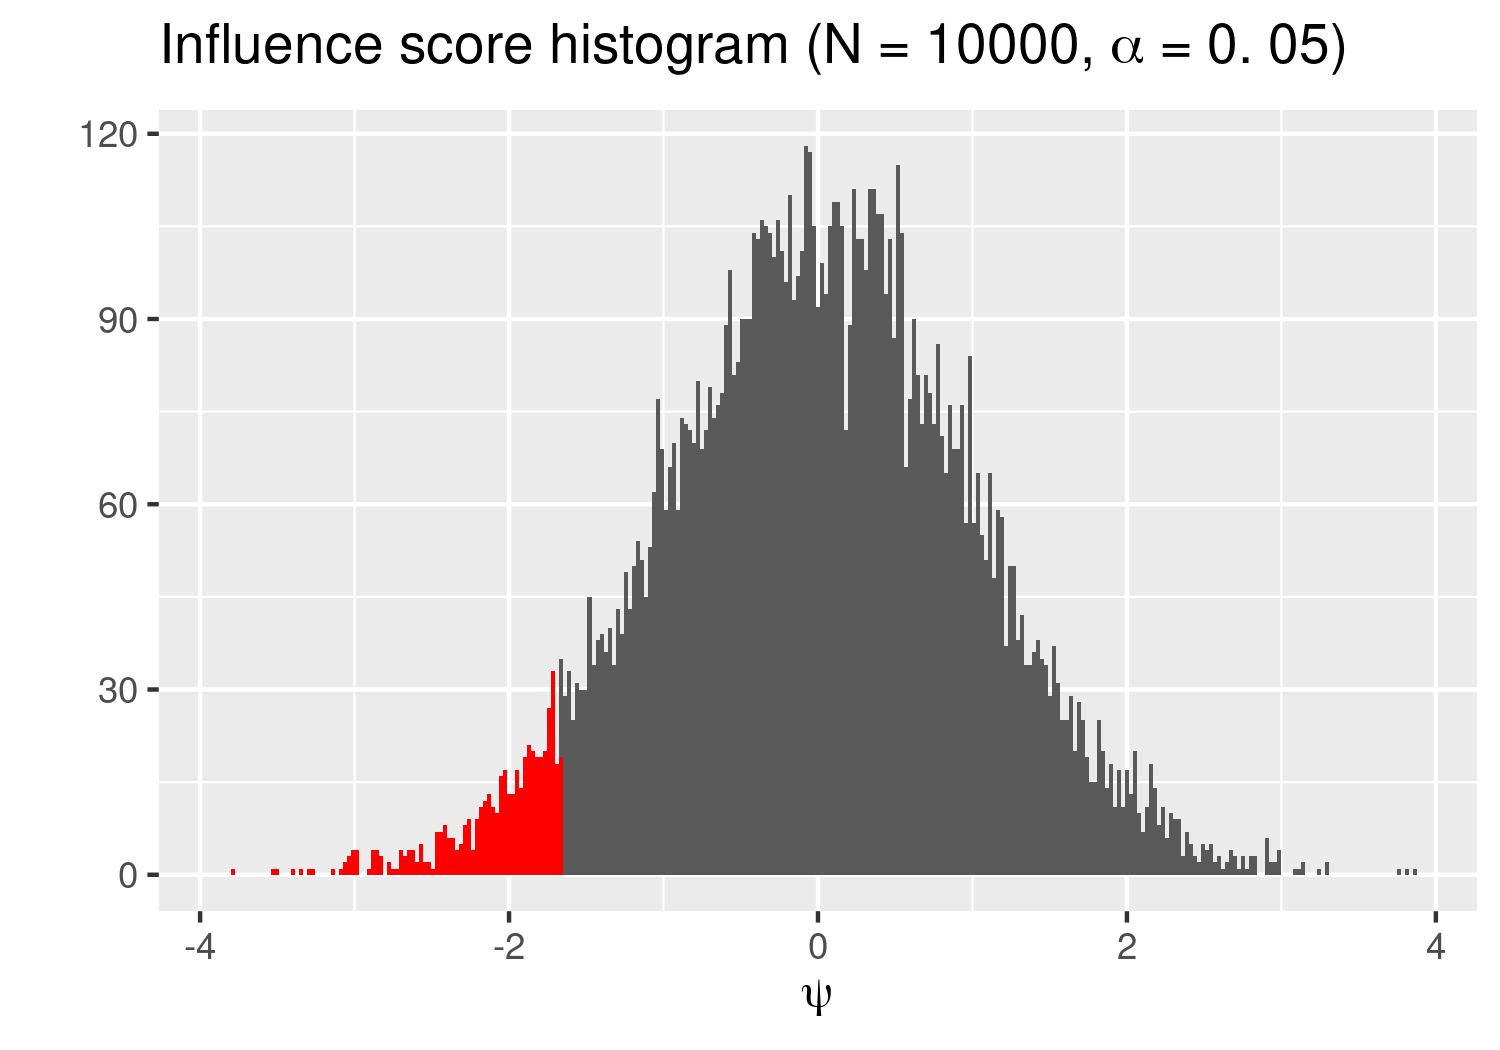
\includegraphics[width=0.98\textwidth]{static_figures/simple_infl_example.png}
    };
    }
    \onslide<3->{
    \begin{scope}[x={(image.south east)},y={(image.north west)}]
        \draw [stealth-stealth][thick][yellow](0.44, 0.4) -- (0.64, 0.4);
    \end{scope}
    \begin{scope}[x={(image.south east)},y={(image.north west)}]
        \draw (0.55,0.38) node[below,yellow][text width=3cm][align=center]
        {\small Controlled by $\var{\sqrt{N}\phi(\thetahat)}$};
    \end{scope}
    }
    \onslide<4->{
    \begin{scope}[x={(image.south east)},y={(image.north west)}]
        \draw [stealth-][thick][red](0.3, 0.25) -- (0.3, 0.5);
    \end{scope}
    \begin{scope}[x={(image.south east)},y={(image.north west)}]
        \draw (0.3, 0.5) node[above,red][text width=3cm][align=center]
        {\small Controlled by Cauchy-Schwartz};
    \end{scope}
    }
\end{tikzpicture}
\end{minipage}
\end{center}

\end{frame}


%%%%%%%%%%%%%%%%%%%%%%%%%%%%%%%%%%%%%%%%%%%%%%%%%%%%%%%%%%%%%%%%%%%%%%%%%
%%%%%%%%%%%%%%%%%%%%%%%%%%%%%%%%%%%%%%%%%%%%%%%%%%%%%%%%%%%%%%%%%%%%%%%%%
%%%%%%%%%%%%%%%%%%%%%%%%%%%%%%%%%%%%%%%%%%%%%%%%%%%%%%%%%%%%%%%%%%%%%%%%%

\begin{frame}{Corollaries.}

{\small
\textbf{Key quantities:}\\
\pause $\alpha$  = The proportion of left out points\\
\pause $\Delta$  = The signal = The change in $\phi$ that would alter your
conclusion\\
\pause $\hat\sigma_\phi^2$ = The noise = A consistent estimator of
$\mathrm{Var}(\sqrt{N}\phi)$\\
\pause $\hat\Gamma_\alpha$ =
The shape = Converges to a nonzero constant, $\le \sqrt{\alpha}$\\
}

\pause
Report non-robustness if the \textbf{``signal to noise ratio''}
$\frac{\Delta}{\hat\sigma_\phi} \le \hat\Gamma_\alpha$.

%\vspace{-1em}

\pause
\vspace{0.5em}
\textbf{Corollary:  Non-robustness possible even with correct specification.}
\vspace{-0.4em}
% {\small The noise $\hat\sigma_\phi$ may be larger than the effect
% $\Delta$ you're trying to measure.}

\pause
\vspace{0.5em}
\textbf{Corollary:  Leave-$\lfloor \alpha N \rfloor$-out robustness does not vanish as $N \rightarrow \infty$.}
% \vspace{-0.4em}
%
% Both $\hat\Gamma_\alpha$ and $\hat\sigma_\phi$ typically converge to nonzero constants.

\pause
\vspace{0.5em}
Recall that standard errors reject when
$\frac{\Delta}{\hat\sigma_\phi} \le \frac{1.96}{\sqrt{N}}$.

\pause
\vspace{0.5em}
\textbf{Corollary:  Leave-$\lfloor \alpha N \rfloor$-out is different from standard errors.}
%\vspace{-0.4em}
% $1.96 / \sqrt{N} \ne \hat\Gamma_\alpha$

% \pause
% \vspace{0.5em}
% \textbf{Corollary:  Insignificance is always non-robust.}
% \vspace{-0.4em}
%
% %Standard errors $\hat\sigma_\phi / \sqrt{N} \rightarrow 0$.
% Take $\Delta = \frac{1.96 \hat \sigma_\phi}{\sqrt{N}} \rightarrow 0 \le
% \hat\Gamma_\alpha$.

% \pause
% \vspace{0.5em}
% \textbf{Corollary:  Gross outliers primarily affect robustness
% through $\hat\sigma_\phi$.}
% \vspace{-0.4em}
%Cauchy-Schwartz is tight when all the influence scores are the same.

\end{frame}



%%%%%%%%%%%%%%%%%%%%%%%%%%%%%%%%%%%%%%%%%%%%%%%%%%%%%%%%%%%%%%%%%%%%%%%%
%%%%%%%%%%%%%%%%%%%%%%%%%%%%%%%%%%%%%%%%%%%%%%%%%%%%%%%%%%%%%%%%%%%%%%%%
%%%%%%%%%%%%%%%%%%%%%%%%%%%%%%%%%%%%%%%%%%%%%%%%%%%%%%%%%%%%%%%%%%%%%%%%


\begin{frame}{Dropping data: Mexico Microcredit}

%\MicrocreditMexicoGraphics{}

% \begin{tabular}{ll}
% { \footnotesize \textbf{Blue line:}}  &       {\footnotesize Original estimate} \\
% { \footnotesize \textbf{Red line:}}  &        {\footnotesize Estimate after removing points} \\
% { \footnotesize \textbf{Shaded bands:}}  &    {\footnotesize Standard errors}
% \end{tabular}

\textbf{Leave-$\alpha$-out robustness does not vanish as $N \rightarrow \infty$.}\\
\textbf{Leave-$\alpha$-out is different from standard errors.}\\
\textbf{Insignificance is always non-robust.}

\end{frame}
